%Papierformat, mit Koma-Script Dokumentenklasse (Europäisches Design)
\documentclass[12pt,a4paper]{scrartcl}
%Deutsche Silbentrennung
\usepackage[ngerman]{babel}
%Listen einrücken
\usepackage{enumitem}
%Deutsche Umlaute
\usepackage[utf8]{inputenc}
%Trennung von deutschen Umlauten
\usepackage[T1]{fontenc}
%Bibtex für Zitate,
% see: https://en.wikibooks.org/wiki/LaTeX/Bibliography_Management#Customization
\usepackage[]{natbib}
%Grafikpaket laden
\usepackage{graphicx}
%Grafik Floating einschränken
\usepackage{placeins}
%Referenzierung mit Name
\usepackage{titleref}
%Unterschritszeilen
\usepackage{tabularx}
%Verlinkung
\usepackage[colorlinks=true,linkcolor=blue]{hyperref}
%Urls sollen erkannt werden
\usepackage{url}
%Ermöglicht es von Schrift umflossene Bilder und Tabellen einzufügen
\usepackage{wrapfig}
%Umbennen der Bibliography Angabe in Literatur
\renewcommand{\bibname}{Literatur}

%\makeatletter
%\newcommand\footnoteref[1]{\protected@xdef\@thefnmark{\ref{#1}}\@footnotemark}
%\makeatother​

%Dokumentbeginn
\begin{document}
	
	\begin{titlepage}
	%Eine mbox wird verwendet um Text zusammenzuhalten
	%vspace erzeugte die in Klammern angegebenen Zeilenabstände
	%baselineskip setzt zeilenabstand
   	\mbox{}\vspace{5\baselineskip}\\
   	%Schriftart und Größe als Attribut
   	\rmfamily\huge
   	%Mittige Textausrichtung (\centerline für eine Zeile)
   	\centering
   	%Das Argument erscheint in Kapitaelchen (small capitals).
	\textsc{Sicherheit in Android und iOS}
	%Umbruch bezogen auf die Hoehe des Kleinbuchstaben x in diesem Element * Faktor
	\\[3ex]
   	Seminararbeit
   	\rmfamily\Large
   	\vspace{1\baselineskip}\\
   	%Externes einbinden einer Textdatei
   	%% versionsnummer entfernt
   	%\input{version.txt}\mbox{}
	\vspace{3\baselineskip}
	Hochschule für angewandte Wissenschaften Würzburg-Schweinfurt
   	\vspace{5\baselineskip}\\
   	\rmfamily\Large
   	David Artmann\\
   	\rmfamily\Large
   	Kristoffer Schneider
   	\vspace{1\baselineskip}\\
   	%Heutiges Datum
   	\today
\end{titlepage}

	%Inhaltsverzeichnis
	\tableofcontents
	\newpage
	
	%Abbildungsverzeichnis
	\listoffigures
	
	%Vorwort
	\newpage
	\section{Vorwort}
	Das Smartphone ist in unserer heutigen Welt nicht mehr wegzudenken. Es dient
	als Alltagshelfer mit vielen Funktionen. Es kann als Notizbuch, oder
	Terminkalender genutzt werden. Es ist eines der Hauptkommunikationsmittel, im
	gesprochenen, als auch geschriebenen Wort. Ebenso wird es auch zum
	Zeitvertreib oder für die Navigation genutzt. Mehrere Studien haben offen 
	gelegt, dass das Smartphone den Computer beziehungsweise Laptop - zumindest
	bei der Generation unter 18 Jahren - schlägt
	\cite{BitkomStudieJugend2014}
	\cite{MPFSStudie2013}.
	Dabei kann leicht vergessen werden, dass Smartphones mittlerweile die Leistung
	eines Bürocomputers haben und die Betriebssysteme dieser Geräte denen von PC
	und Laptop immer ähnlicher werden. Daraus ergeben sich für mobile Geräte
	ähnliche Gefahren wie für Computer und Laptop. Ein einfacher Vergleich:
	Anti-Viren Software ist auf den klassischen Computersystemen weit verbreitet,
	aber wer nutzt eine solche Software auf seinem Smartphone oder Tablet? Dabei
	sind auch auf diesen Geräten hoch sensible Daten gespeichert.\\
	Mit dieser Arbeit soll die Sicherheitsarchitektur der mobilen Betriebsysteme
	iOS und Android vorgestellt und erläutert werden. Weiterhin werden die
	Fähigkeiten beider Systeme in Bezug auf Gewährleistung dieser Sicherheit,
	sowohl auf Betriebsystem- als auch Applikationsebene beleuchtet.

	
	%Das Android Betriebssystem 
	\newpage
	\subsection{Android}
	Das Unternehmen Android wurde 2003 von Andy Rubin gegründet und wurde 2005 von
	Google aufgekauft. Seitdem hat Google und das Android Open Source Project
	(AOSP) die Weiterentwicklung des Systems übernommen. Zuletzt wurden die neuen
	Versionen jeweils von Google intern entwickelt und zum Release der Version der
	AOSP Community als Open-Source bereitgestellt. Das Betriebssystem wird in den
	meisten Fällen von den Smartphone Herstellern oder Entwicklerteams noch weiter
	angepasst, bevor es für die einzelnen Geräte bereitgestellt wird.\\
	Basis für das Betriebssystem ist ein modifizierter Linux-Kernel und eine Java
	Virtual Machine (JVM) \cite{ArtDalvik}. Bis einschließlich Version 4.4 wurde
	hierfür die Dalivk Runtime und für alle neueren Versionen die Android Runtime
	(ART) verwendet. Jede App l"auft in einer eigenen Instanz der entsprechenden
	Runtime und in einer Sandbox. Oberhalb der JVM sind die meisten Komponenten in
	Java implementiert.
	\begin{figure}[h]
		\centering
		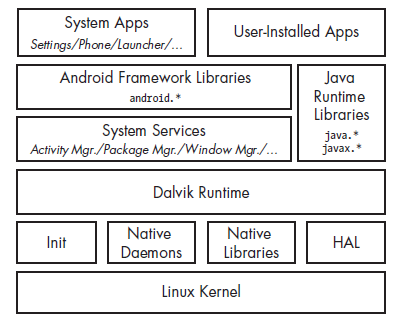
\includegraphics[width=0.7\linewidth]{android_pages/graphics/architektur_android_.png}
		\caption{Die Android Architektur \protect\cite[S. 2]{Elenkov2014} }
		\label{fig:architektur_android}
	\end{figure}
	\\\\
	\textbf{Die Dalvik- und Android Runtime}\\
	Ein grundsätzlicher Unterschied zwischen einer klassischen JVM, wie sie auf
	dem Desktop und anderen Geräten zum Einsatz kommt, und einer Runtime die auf
	Android läuft ist der, dass auf Android die Runtime auf einer Register-
	anstatt auf einer Stackmaschine basiert \cite{DalvikBytecode}. Somit
	unterscheidet sich der Bytecode zwischen den Plattformen. Eine
	Registermaschine bringt mehrere Vorteile mit. Unter anderem ist der Bytecode
	kleiner, was gerade mobilen Endgeräten entgegen kommt.
	Zusätzlich wird nicht mehr mit den üblichen \textit{jar}- und
	\textit{class}-Dateien, sondern mit einem eigenen Format namens \textit{.dex}
	gearbeitet \cite{DexFormat}. Dieses ist für den mobilen Einsatz optimiert.\\
	Die Dalvik Runtime stammt noch aus dem ursprünglichen Android Projekt und
	ähnelt einer klassischen JVM noch sehr. Sie interpretiert Bytecode zur
	Laufzeit und ist in der Lage oft genutzten Code zur Laufzeit zu kompilieren
	(\textit{Just-in-time-Compilation, kurz: JIT}).
	Die größte Änderung mit dem Umstieg auf die Android Runtime ist, dass nun
	vorkompilierter Programmcode (\textit{Ahead-Of-Time-Compilation}, kurz:
	\textit{AOT}) genutzt wird. Der Hintergrundgedanke dieser Veränderung ist,
	dass dadurch die Performance deutlich verbessert wird. Allerdings ist nativ
	kompilierter Code größer als Bytecode, wodurch wiederum mehr Speicher auf den
	Geräten benötigt wird. Da Android auf vielen verschiedenen Hardware
	Plattformen ausführbar sein muss und der native Code plattformabhängig ist,
	wird der Bytecode während der Installation in Nativen kompiliert.\\
	Durch das Nutzen von Java wird Exploits, welche auf Basis von Bufferoverflows
	arbeiten, entgegen gewirkt, da Java die Speicherzugriffe überprüft und bei
	Überläufen eine Exception wirft, was den Abbruch der auslösenden Operation als
	Folge hat. Dieser Schutz ist allerdings nur unter der Nutzung von
	Java-Programmcode vorhanden und nicht wenn nativer, z.B. durch den Einsatz des
	Java-Native-Interfaces (\textit{JNI}), genutzt wird.

	
	%Das iOS Betriebssystem
	\newpage
	\subsection{iOS}
	Die aus Cupertino in Kalifornien stammende US-Amerikanische Apple Corporation
	besitzt weltweit den größten Marktwert mit 741,8 US-Dollar und einen
	Umsatz von 199,4 Milliarden US-Dollar im laufenden Geschäftsjahr 2015 laut der
	in den Forbes Global 2000 aufgelisteten Unternehmen \cite{FORBES2000}.
	Sie ist der Erfinder des mobilen Betriebssystems iOS, welches auf den firmeneigenen Geräten iPad, iPad mini,
	iPhone, iPod touch und dem Apple TV ab der zweiten Generation zum Einsatz
	kommt. Als Steve Jobs 1985 das Unternehmen verließ, gründete er
	kurze Zeit darauf die Firma NeXT, mit welcher er unter anderem das
	Betriebssystem NeXTStep entwickelte, welches auf dem UNIX ähnlichem
	Betriebssystem BSD \cite[S.12]{Tanenbaum2009} und dem
	Mach-2.5-Kernel \cite{MachProject2015} basiert. NeXT wurde 1996 von Apple
	aufgekauft und Jobs kehrte als CEO zu Apple zurück. Damit begann die Karriere
	des mobilen Betriebssystems iOS. Zuerst wurde NeXTStep als Portierung in Form
	von Mac OS X (später OS X) weiter entwickelt. Mac OS X ist wiederrum der
	Vorleger für das iPhone OS (später iOS), welches am 09. Januar 2007 mit dem
	damals neu erschienenen iPhone erstmals vorgestellt wurde.
	\\\\
	\textbf{Apple's Law Enforcement Process Guidelines}
	\\
	Die Firma Apple schreibt auf ihrer Webseite:
	\begin{quote}
		Our commitment to customer privacy doesn't stop because of a government
		information request \cite{AppleGovInfo2015}.
	\end{quote}
	Weiterhin wird beteuert:
	\begin{quote}
		In addition, Apple has never worked with any government agency from any
		country to create a "`back door"' in any of our products or
		services \cite{AppleGovInfo2015}.
	\end{quote}
	Apple beteuert hier, die Privatssphäre des Kunden auch dann zu bewahren,
	wenn die Regierung um Auskunft der Daten bittet.\\
	Zusätzlich wird versichert, dass Apple niemals mit Regierungsbehörden
	jedweder Länder gearbeitet hat, um Trojaner oder andere Hintertüren in eines
	ihrer Produkte oder Dienstleistungen einzubauen.\\
	Grundsätzlich ist eine Einhaltung dieser Versprechen wünschenswert, sowohl für
	Entwickler als auch Endnutzer, da beide Parteien über die proprietäre
	Vorgehensweise, Apple in gewisser Art und Weise vertrauen müssen.

	
	%Apple's law enforcement process guidelines
	\newpage
	\section{Apple's Law Enforcement Process Guidelines}
	Die Firma Apple schreibt auf ihrer
	Webseite:
	\begin{quote}
		Our commitment to customer privacy doesn't stop because of a government
		information request.\cite{AppleGovInfo2015}
	\end{quote}
	Weiterhin wird beteuert:
	\begin{quote}
		In addition, Apple has never worked with any government agency from any
		country to create a "`back door"' in any of our products or
		services.\cite{AppleGovInfo2015}
	\end{quote}
	Apple beteuert hier, seine Verpflichtung zur Einhaltung der Privatssphäre des
	Kunden auch nicht einzustellen, wenn die Regierung um Auskunft genau dieser
	Daten bittet.\\
	Zusätzlich wird versichert, dass Apple niemals mit Regierungsbehörden
	jedweder Länder gearbeitet hat, um Trojaner oder andere Hintertüren in eines
	ihrer Produkte oder Dienstleistungen einzubauen.

	
	%Grundlegender Aufbau einer Android App
	\newpage
	\subsection{Android}\label{sec:app-android}
	\begin{quote}
	Android apps are written in the Java programming language. The Android SDK tools compile your code - along with any data and resource files - into an APK: an \textit{Android package}, which is an archive file with an .apk suffix. One APK file contains all the contents of an Android app and is the file that Android-powered devices use to install the app.\cite{AndroidApp}
	\end{quote}
	
\begin{flushleft}
	Applikationen werden zumeist in Java oder C/C++ geschrieben; selten kommen auch andere JVM-Sprachen zum Einsatz.
	Eine Android App besteht im Kern unter anderem aus zwei wichtigen Teilen: den eigentlichen Programmkomponenten und einer Manifest Datei (AndroidManifest.xml).\\
\end{flushleft}
	\subsubsection{Programmkomponenten}
	Als Programmkomponenten können unter anderem vorkommen:
	\begin{itemize}\itemsep0pt
		\item Activities - stellen die Benutzeroberfläche dar
		\item Services - kann im Hintergrund laufen, auch wenn die App minimiert ist
		\item Content Provider - stellt Daten für die eigene und evtl für andere Apps zur Verfügung
		\item Broadcast Receiver - um Systemweite Benachrichtigungen zu empfangen (z.B dass ein Download beendet wurde)
	\end{itemize}
	\subsubsection{Manifest-Datei}
	In der Manifest-Datei werden Eigenschaften der App definiert. Darunter zählen beispielsweise:
	\begin{itemize}\itemsep0pt
		\item Name der App
		\item Ziel SDK-Versionen
		\item Versionsnummer
		\item optional eine UserId (Kapitel \ref*{sec:BasisRechteSystem})
		\item Permissions (Kapitel \ref*{sec:SandBoxingNPermissions})
		\item Startpunkt der Applikation
	\end{itemize}
	\subsubsection{Signatur}
	Jede App muss signiert werden. Das hierfür benötigte Zertifikat kann sich jeder Entwickler selbst generieren und muss nicht durch eine Certification Authority (CA) beglaubigt werden. Dabei wird angeraten, dass ein Entwickler für all seine Apps dasselbe Zertifikat nutzt. Mithilfe der dadurch gegebenen Signatur wird eine \textit{Same-Origin-Policy} erschaffen, die bei jedem Update sicherstellt, dass dieses wirklich vom Entwickler der Applikation stammt und nicht durch Dritte eingebracht wurde.\\\\
	Hauptquelle für Anwendungen der Android Plattform ist der \textit{Google Play Store}. Mittlerweile gibt es allerdings auch andere vertrauenswürdige Quellen, z.B. Amazons \textit{App Shop}.
	
	\subsubsection{Entwicklung}
	Java als Programmiersprache bringt mehrere Vorteile mit sich. Mit die wichtigsten sind, dass Java leicht zu lernen ist, was sich entsprechend auch auf die Anzahl der Apps für Android niederschlägt. Auch gibt es eine große Anzahl an Entwicklungsumgebungen, die oftmals sogar kostenlos nutzbar sind.\\
	Dass Apps somit schnell programmiert werden können, kann allerdings auch ein Nachteil sein, z.B. wenn Entwickler aufgrund von Unwissen Nutzerdaten nicht korrekt schützen, oder sogar versehentlich eine Sicherheitslücke zur Verfügung stellen.
	
	%Sicherheitsarchitektur iOS
	\newpage
	\section{Komponenten der Systemsicherheit unter
iOS}\label{sec:components-syssec} 
	Eine Kette von aneinander gereihten und von einander abhängigen Prozessen trägt
	maßgeblich zur Systemsicherheit von iOS bei. Dies berücksichtigt vor allem den
	Startvorgang, die Softwareupdates - auch von Drittanbietern - und den Secure
	Enclave (Kapitel \ref{sec:secure_enclave}). Dies stellt sicher, dass
	alle Kernkomponenten, ob Hard- oder Software, möglichst gefeit vor Angriffen sind,
	ohne dabei die Nutzerfreundlichkeit zu beeinflussen. Wenn dabei einer dieser
	Schritte fehlschlägt, unterbricht der Startvorgang und das Gerät wird in den
	Recovery Modus versetzt. Wenn der Boot-ROM nicht geladen werden kann, wird der
	DFU\footnote{Device Firmware Upgrade: DFU} Modus
	betreten.\\
	Nachfolgend werden die Komponenten, welche maßgeblich zur Wahrung der
	Systemsicherheit und der Integrität dieser beteiligt sind, detailliert
	vorgestellt und beschrieben.
	
	\begin{figure}[h]
		\centering
		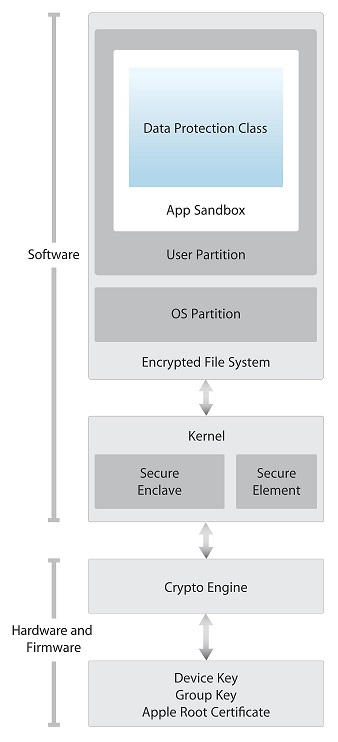
\includegraphics[width=0.4\linewidth]{ios/media/security-model.jpg}
		\caption{Sicherheitsmodel von iOS 
		\cite[S.4]{iOSSecurityApr2015}}
		\label{fig:security-model}
	\end{figure}

	%TODO: look at learning ios security, there this whole process is explained
	% good
	\subsection{Secure boot chain}\label{sec:secure-boot-chain}
		Dieses Verfahren stellt eine Manipulation der Low-Level Software sicher. Nur
		iOS Geräte, deren Vertrauenskette erfolgreich validiert wurde, starten
		ordnungsgemäß. Dabei wird nach dem Start eines iOS Gerätes zuerst Code aus
		einem nur lesbaren Speicherbereich ausgeführt. Dieser \textit{hardware of
		trust} genannte und unveränderbare Code ist bei der Manufaktur der Chips
		eingebettet worden und somit implizit vertraulich. Das Boot ROM enthält
		zusätzlich den öffentlichen Schlüssel der Wurzel Zertifizierungsstelle von
		Apple, welcher eine Signierung des Low-Level-Bootloaders durch Apple sicher
		stellt, bevor er ausgeführt wird.
		Dies ist der erste Schritt in der "`chain of trust"', in welcher jeder
		Teilnehmer sicher stellt, dass der darauf folgende von Apple signiert ist. 		
		Nach erfolgreicher Abarbeitung aller Aufgaben des LLB, überprüft und startet
		dieser iBoot, den nächsten Bootloader, welcher wiederrum das selbe Prozedere
		mit dem iOS Kernel beginnt. Bei Geräten mit Mobilfunk Zugang führt das
		Basisband Untersystem seinen eigenen ähnlichen Prozess mit signierter 
		Software und verifizierten Schlüsseln des Basisband Prozessors durch.
		
	\subsection{Authorisierung von System Software}\label{sec:code-signing}
		Dieser Prozess soll einen Downgrade auf eine ältere Version von iOS
		verhindern. Der im folgenden Kapitel besprochene Secure Enclave Co-Prozessor
		nutzt diese Technik für Integritätsprüfung seiner Software ebenfalls. Im Falle
		eines iOS Updates wird entweder von iTunes oder vom Gerät selbst einer der
		autorisierenden Installationsserver von Apple kontaktiert. Diesem
		wird eine Liste von verschlüsselten Informationen pro am Update beteiligter
		Komponente gesandt. Zusätzlich wird ein zufälliger
		%TODO: add long version of ECID
		Anti-Replay Wert und die eindeutige ID des Gerätes
		verschickt. Die Clientdaten werden gegen eine Auflistung authorisierter Hardware, für die ein
		Update genehmigt sind geprüft. Bei Übereinstimmung wird die
		ECID\footnote{Eindeutige ID: ECID} zu den Informationen hinzugefügt und das
		Ergebnis signiert, was einer Personalisierung der Daten gleicht.
		Anschließend werden alle nötigen Daten vom Server signiert und zum Gerät
		geschickt. Die sichere Startkette von Prozessen (Kapitel
		\ref{sec:secure-boot-chain}) verifiziert die Signatur der empfangenen Daten
		auf den Absender Apple und gleicht die Prüfsumme der Signatur mit dem lokalen
		Ergebnis von verschlüsselten Informationen und ECID ab.\\
		Mit diesen Schritten wird eine Authorisierung ausschließlich für authorisierte
		Geräte sicher gestellt. Außerdem verhindert der Anti-Replay Wert ein
		Manipulieren der Serverdaten, oder ein Mitschneiden dieser für
		das Verwenden auf anderen, nicht authorisierten Geräten.
	\subsection{Secure Enclave}\label{sec:secure_enclave}
		%TODO: get more details for ensuring the facts in this chapter
		Dieser Co-Prozessor kommt in Geräten mit A7 oder jüngeren A-Serien Prozessoren
		vor. Er verwendet seinen eigenen sicheren Startvorgang, ist separiert vom
		Applikations Prozessor und verwendet verschlüsselten Speicher, sowie einen
		Hardware Zufallszahlen Generator. Die Technologie basiert auf ARM's
		TrustZone\cite{TrustZone2015}
		und wurde von Apple für die eigenen Ansprüche angepasst. Der Kernel dieser
		Einheit basiert auf der L4
		Mikrokernel-Familie\cite{L4MicroKernel2015} mit leichten
		Modifikationen. Die auf Interrupts basierende Kommunikation zwischen dem
		Applikationsprozessor und dem Secure Enclave läuft über einem nur den beiden zur Verfügung stehenden Speicherbereich.
		Der SE\footnote{SE: Secure Enclave} ist verantwortlich für das Schlüssel
		Management der Datenverschlüsselung und stellt die Integrität dieser sicher, auch wenn der
		Kernel des iOS Systems kompromitiert ist. Beim Herstellungsprozess erhält
		jeder SE eine einzigartige ID, auf welche nur er zugreifen kann. Selbst Apple,
		oder anderen an der Produktionskette beteiligten Herstellern ist diese nicht bekannt.
		Mit dieser UID\footnote{Einzigartige ID: UID} wird beim Systemstart der
		Speicherbereich des SE zusammen mit einem einmaligen Schlüssel verschlüsselt.
		Zusätzlich werden jegliche vom SE in den Speicher geschriebene Daten mit der
		UID und einem Anti-Replay Zufallswert verschlüsselt. Eine der Hauptaufgaben
		des Secure Enclave ist die verarbeitung der Fingerabdruck-Daten des Touch ID
		(Kapitel \ref{sec:touch_id}).
		Alle Kommunikation zwischen Touch ID und SE wird über einen seriellen Bus
		abgearbeitet. Der Applikationsprozessor leitet die Fingerabdrucksdaten an den
		SE weiter kann diese aber aufgrund einer Verschlüsselung der Daten mit einem
		Sitzungsschlüssel nicht lesen. Dieser Session Key wurde durch den für Touch
		ID und SE bereit gestellten öffentlichen Schlüssel erzeugt. Der Austausch des
		%TODO: long form of AES in footmark
		Sitzungsschlüssels wird durch AES Key Wrapping realisiert. Dabei erzeugen
		beide Seiten einen zufälligen Schlüssel, welche den Sitzungsschlüssel bilden.
		%TODO: long form of AES-CCM in footmark
		Zum verschlüsselten Transport wird AES-CCM genutzt.
	\subsection{Touch ID}\label{sec:touch_id}
		Touch ID bezeichnet den Fingerabdrucksensor der in allen iPhone 5s und neuer
		, sowie iPad Air 2 und iPad mini 3 verbaut ist. Es können bis zu 5
		%TODO: check if advantage is the locking or maybe ENCRYPTION, when s/w-button
		% is pressed
		Fingerabdrücke gespeichert werden. Eine der größten Vorteile dabei ist das
		sofortige Sperren des Gerätes beim drücken des Sleep/Wake-Buttons. Dies gilt
		auch bei aktiviertem Passcode. Vor der Einführung von Touch ID haben viele
		%TODO: details of Passcode in footmark, or in sentence after mention it?
		Nutzer eine möglichst lange Zeit eingestellt, bis das Eingeben des Passcodes
		nötig wurde, nachdem das Gerät gesperrt wurde. Dies entfällt nun bei
		aktivierter Touch ID, da der Nutzer nur noch mit seinem Finger Entsperren
		muss.
		Touch ID kann zusätzlich zum Entsperren des Gerätes auch mit dem Zahlungsdienst Apple
		Pay und für Einkäufe in iTunes, dem App Store und im iBook Store genutzt
		werden. Für Entwickler steht eine API bereit mit der rudimentärste
		Prüfungen auf erfolgreiche Verifikation des Abdrucks erfolgen können. Ein
		direkter Zugriff auf Touch ID oder die Daten des Fingerabdrucks wird von
		Apple unterbunden. Touch ID wird aktiviert, wenn der kapazitive Stahlring um
		den Sensor einen Fingerdruck wahrnimmt. Anschließend wird dieser gescannt und
		an den Secure Enclave gesandt. Der Abdruck wird kurzzeitig im veschlüsselten
		%TODO: better description?!
		Speicher des SE für eine Vektorisierung der Fingerabdruckdaten gespeichert, um
		danach verworfen zu werden. Die Schlüssel, welche von Touch ID zum
		Entschlüsseln des Gerätes benötigt werden, sind nach 48 Stunden ungültig,
		beziehungsweise wenn das iOS Gerät neu gestartet wurde, oder der
		Fingerabdruck fünf mal falsch registriert wurde.\\
		Dass diese Technik nicht als Sicher angesehen werden darf, haben bereits
		Miglieder des Chaos Computer Club gezeigt\cite{CCCBreakTouch2015}, dabei 
		wurde mit simpelsten Haushaltsmitteln ein Fingerabdruck gefälscht, den das
		Smartphone irrtümlicher weise akzeptiert hat.

	\section{Verschlüsselung unter iOS}
	In diesem Kapitel werden die Kryptographie von iOS genauer vor gestellt.
	Dazu werde ich erst auf eingesetzt Hardware eingehen und dann auf die logische
	Ebene wechseln mit einem Fokus auf Dateizugriff.
	\subsection{Kryptographische Hardware}\label{sec:crypto-engine}
		Für eine native Verschlüsselung sorgt in jedem iOS Gerät eine AES256 bit
		basierte Hardware-Engine, welche zwischem dem Flash	Speicher und dem
		Systemspeicher liegt. Diese Positionierung sorgt für hohe Performance und
		niedrige Latenzen beim Verschlüsseln von Dateien. Die geräteeigene Unique ID
		(UID) wird beim Herstellungsprozess in den Applikationsprozessor und den Secure
		Enclave eingebrannt und die Group ID (GID) wird compiliert, somit ist es keiner
		Soft- oder Firmware möglich diese direkt zu lesen. Dies verhindert eine
		Manipulation oder ein Umgehen dieser Schlüssel, sowie einen Zugriff außerhalb
		der Krypto-Engine. Die UID erlaubt außerdem eine Gerätspezifische Bindung von
		Daten.
		Apple beteuert unter anderem
		\begin{quote}
			The UIDs are unique to each device and are not recorded by Apple or any of its
			suppliers.\cite[S.9]{iOSSecurityApr2015}
		\end{quote}
		Die GID hingegen ist allen Geräten einer Prozessorklasse bekannt, z.B. all
		jenen die einen Apple A7 nutzen. Dies liegt an der weniger
		Sicherheitskritischen Nutzung dieser Schlüssel für Vorgänge,
		wie beispielsweise die Übertragung von System Software bei Updates. Jegliche
		weitere bei Kryptografischen Operationen benötigte Schlüssel werden von einem
		Random Number Generator (RNG) mit einem auf	CTR\_DRGB
		\footnote{http://csrc.nist.gov/publications/nistpubs/800-90A/SP800-90A.pdf}
		basierendem Algorithmus erzeugt.
	\subsection{Schutz auf Dateiebene}
		Zusätzlich zur Hardwareverschlüsselung nutzt iOS ein Feature namens \textsl{Data
		Protection} um Daten auf dem Flash Speicher zu schützen. Dieser Mechanismus
		wird bei allen System Apps und ab iOS7 auch bei Drittanbieter Apps
		automatisch angewendet. Die Funktionsweise ist Form einer Schlüsselhierarchie
		im Verbund mit Hardwareverschlüsselung realisiert. Jede Datei, die in den
		Speicher geschrieben wird, erhält einen 256 Bit explizit ihr zugewiesenen
		\textsl{Per-File} Schlüssel. Dieser wird von der
		%TODO: get infos about AES-CBC + the initialization vector
		Verschlüsselungsengine (siehe: \ref{sec:crypto-engine}) mit Hilfe von
		AES Cipher Block Chaining verschlüsselt. Der Per-File Schlüssel wird mit
		einem von vier Klassenschlüsseln ummantelt und in den Meta-Daten gespeichert.
		Der Klassenschlüssel ist zusätzlich noch mit der UID und für manche auch mit
		dem Passcode des Benutzer gesichert. Jegliche Meta-Daten sind mit einem
		zufälligen Schlüssel verschlüsselt, welcher beim installieren von iOS oder
		beim Löschen eines Gerätes durch den Benutzer erstellt wird. Beim
		Entschlüsseln einer Datei, werden zuerst die Meta-Daten mit dem \textsl{File
		System Key} entschlüsselt. Dieser ist im \textsl{Effaceable Storage}
		gespeichert - einem dedizierten Bereich im NAND-Speicher, welcher direkt
		adressiert und sicher gelöscht werden kann.
		Sobald dieser Speicher und somit der darin enthaltene Dateisystem Schlüssel
		gelöscht wurde, macht dies alle Dateien auf dem Gerät kryptografisch
		unwiederherstellbar. Sobald der Benutzer einen Passcode auf dem System
		einrichtet, aktiviert er Data Protection.
		\begin{figure}[h]
			\centering
			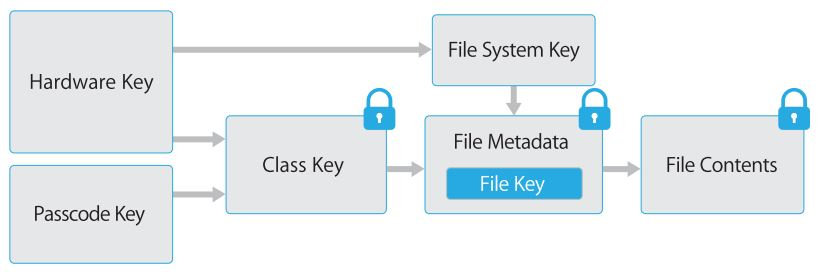
\includegraphics[width=0.9\linewidth]{ios/media/data-protection.jpg}
			\caption{Data Protection Architektur 
			\cite[S.10]{iOSSecurityApr2015}}
			\label{fig:data-protection}
		\end{figure}

	
	%Sicherheit Android
	\newpage 
	\section{Sicherheitsaspekte der Android-Architektur}

	Bereits durch die Architektur des Betriebssystems, insbesondere durch die restriktive Rechtevergabe und das Sandboxing, wird versucht, ein möglichst sicheres System bereitzustellen. Ab Android Version 4.3 kommt zusätzlich noch \textit{Security-Enhanced Linux (SELinux)} zum Einsatz.\\
	Verschlüsselungen und Signaturen werden Hardwareseitig durch eine \textit{Trusted Execution Environment (TEE)} unterstützt. TEE stellt einen besonders geschützten Bereich auf dem Prozessor dar, auf dem nur berechtige Anwendungen ausgeführt werden können, wie beispielsweiße die Verifikation des Bootmediums und Verschlüsselungsverfahren. Die Implementierung ist dabei Prozessor Hersteller abhängig - auf ARM wird dabei, wie bei iOS, auf \textit{TrustZone}\cite{TEE_ARM} zurückgegriffen.
	
	\subsection{Verifikation der Bootmedien} \label{sec:VerifikationDerBootmedien}
	Um bereits bei Systemstart eine Veränderung oder Ersetzung der Paritionen zu erkennen, wurde mit Android 4.4 eine Boot Verification eingeführt. Das Verfahren basiert auf der Funktion dm-verity des Device Mappers, welcher im Linux Kernel zu finden ist. Da diese Überprüfung durch den Kernel ausgeführt wird, muss vor dem Start von dm-verity erst der Bootloader und die Boot-Partition selbst auf ihre Integrität überprüft werden.
	Die Verifikation des Bootloaders ist nur schwer möglich, daher wird hierbei auf eine Hardware basierende root-of-trust, hier auf Basis des TEE, gesetzt. \\
	
	\subsubsection{Integritätscheck durch den Bootloader}
	Grundsätzlich ist Implementierung des Bootloader und dessen Vorgehen stark Geräteabhängig, daher werde ich hier im Folgenden lediglich das prinzipielle Vorgehen, welches durch das AOSP unterstützt wird, erläutern.\\
	Um die Boot- und Recovery-Partition (\textit{/boot, /recovery}) zu validieren gibt es zwei Möglichkeiten. Ist auf den beiden Partition jeweils ein offizielles Images des Smartphone Herstellers, kann auf einen OEM Key zurückgegriffen werden. Dieser ist in einem read-only in der Hardware festgeschrieben und wird vom Hersteller des Systems - zumeist der Smartphone Hersteller - festgelegt. Sollte eine Veränderung des Images vorgenommen worden sein, egal ob bewusst durch den Nutzer oder durch Schadcode, ist dieses Vorgehen nicht mehr möglich. Um aber dennoch eine Modifikation durch den Nutzer grundsätzlich zu ermöglichen, gibt es noch eine zweite Möglichkeit. Dabei wird auf ein, in der Paritionssignatur gespeichertes, Zertifikat zurückgegriffen.\\\\
	Um zu unterscheiden ob ein offizielles oder inoffizielles Image erwartet wird, kann der Bootloader zwischen zwei Status unterscheiden:\\
	
	\begin{itemize}\itemsep0pt
		\item LOCKED - das aktuelle Boot-Image ist ein offizielles und kann mittels OEM Key verifiziert werden
		\item UNLOCKED - das aktuelle Boot-Image wurde verändert, und kann daher nicht mit dem OEM Key veriiziert werden
	\end{itemize}
	
\begin{flushleft}
	Diese und andere Informationen sind zwischen verschiedenen Images weites gehend gleich und werden daher auf einer extra Partition gespeichert (zumeist \textit{/misc} oder \textit{/param}), welche somit im Falle eines Wechsel des Images nicht neu aufgesetzt werden muss.
\end{flushleft}
	 Wurde dies getan, wird beim Hochfahren immer eine Warnung ausgegeben, um den Nutzer darauf hinzuweisen, dass die Partition nicht mittels des festgeschrieben Keys verifiziert werden konnte. Daraus ergeben sich mehrere mögliche Zustände des Systems:\\\\
	
	\begin{figure}[h]
		\centering
		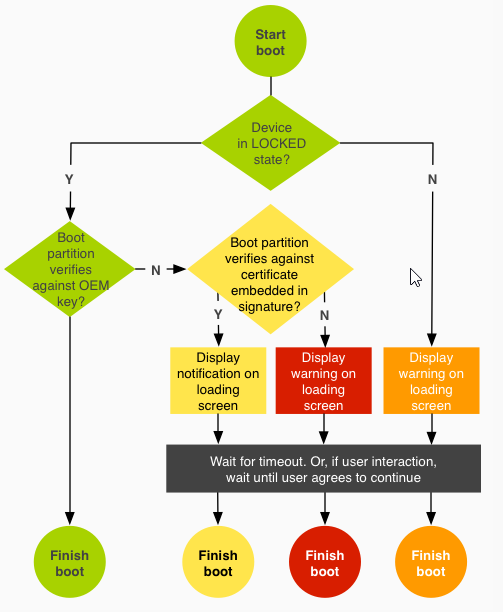
\includegraphics[width=0.7\linewidth, height=0.5\textheight]{android_pages/graphics/VerifiedBoot}
		\caption[Verified boot flow\protect\cite{VerifyingBoot}]{Verified boot flow\protect\cite{VerifyingBoot}}
		\label{fig:VerifiedBoot}
	\end{figure}
	
\begin{flushleft}
	Mit diesem Vorgehen wird auch die Integrität des Kernels sichergestellt, welcher in der \textit{/boot-} Partition abgelegt ist. Die Steuerung wird nach diesem Vorgang an den Kernel übergeben, welcher die Verifikation weiterer Partitionen übernimmt.\newline\\

	Um zu verhindern, dass Angreifer einfach den Bootloader manipulieren um an Daten heranzukommen, muss die Partition welche die Nutzerdaten beinhaltet (\textit{/userdata}) vor einer Veränderung an dem Bootsystem formatiert werden.
\end{flushleft}
	
	\subsubsection{Integritätscheck weiterer Paritionen}
	Weitere Integritätschecks werden von der Kernelfunktion dm-verity übernommen.
	dm-verity arbeitet mit einem SHA-256 Hash-tree, der wie folgt aufgebaut ist:\\
	Für jeden 4K Sektor auf der Parition wird ein Hashwert berechnet. Jeweils zwei dieser Werte werden wiederum zu einem Neuen verrechnet. Dies wird solange wiederholt, bis nur noch ein Hashwert, der \textit{root-hash}, übrig ist. Um nun die Integrität sicherzustellen wird dieser root-hash, mit einem bereits berechneten Soll-Wert verglichen. Sind diese identisch, ist die Parition integer.
	
	\begin{figure}[h]
		\centering
		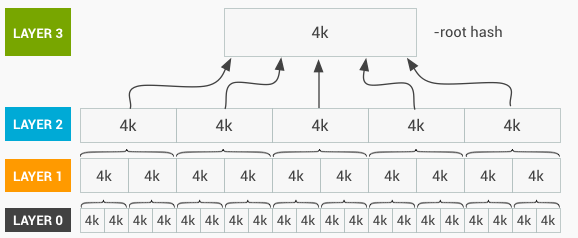
\includegraphics[width=0.7\linewidth]{android_pages/graphics/dm-verity-table}
		\caption[Aufbau des Hash-Trees]{Aufbau des von dm-verity erstellten Hash-Trees\protect\cite{VerifiedBoot}}
		\label{fig:dm-verity-table}
	\end{figure}
	
\begin{flushleft}
	Um Manipulationen am Soll-Wert zu unterbinden, wird der Hash-Tree und ein Salt mit einem RSA Schlüssel signiert. Der genutzte RSA Public Key wird in der Boot-Partition abgelegt. Der Hash-Tree und der Salt hingegen werden hinter dem letzten Datenblock auf die zu verifizierenden Partitionen geschrieben. Besonders geeignet ist dieses Verfahren für Read-Only Paritionen, wie die System-Partition welche das Betriebssystem beherbergt.\\
	Welche Paritionen mittels vm-verity auf ihre Integrität überprüft werden sollen, wird über einen Eintrag zu der jeweiligen Partition in der fstab-Datei festgelegt.
\end{flushleft}

	\subsection{Basis Rechtesystem}\label{sec:BasisRechteSystem}
	Von Linux wurde auch das Basis-Rechtesystem Übernommen, allerdings wird es leicht abgewandelt genutzt. Anstatt das ein Nutzer des Mobilsystems eine eindeutige User-ID (UID) zugewiesen bekommt, wird jede Applikation auf dem System als ein Nutzer angesehen und bekommt zur Installationszeit eine UID. Jeder Nutzer, und somit auch jede App, arbeitet grundsätzlich erst einmal nur innerhalb der ihm zugewiesenen virtuellen Maschine und dem damit verbundenen Dateisystem.\\\\
	Da es dennoch in vielen Fällen nötig ist, Daten zwischen verschiedenen Apps auszutauschen, gibt es mehrer Möglichkeiten dies zu tun. Die üblichen Wege wären Intends oder Contentprovider. Zusätzlich gibt es noch die Möglichkeit mehreren Apps dieselbe UID zuweisen zu lassen. Dies ist allerdings nur möglich, wenn die entsprechenden Applikationen mit dem selben Zertifikat signiert wurden und in deren Manifest Datei eine gemeinsame UID festgelegt wurde.
	Durch dieses Rechtesystem wird versucht sicherzustellen, dass kein Nutzerprogramm als \textit{root} ausgeführt wird.
	
	\subsection{Sandboxing und Permissions} \label{sec:SandBoxingNPermissions}
	Wie bereits erwähnt, laufen die Applikationen jeweils in ihrer eigenen Sandbox. Grundsätzlich ist die App damit in ihrer Ausführung auf ihren Bereich beschränkt und kann nicht mit anderen Prozessen und Daten ausserhalb interagieren. Dennoch ist es in den meisten Fällen sinnvoll mit Systemservices und Nutzerdaten zu interagieren, die nicht in der eigenen Sandbox verfügbar sind. 
	
	\subsubsection{Sandboxing}
	Das Sandboxing in Android basiert auf dem Rechtesystem des Linux-Kernels und der JVM. Prozesse eines Nutzer können nicht den Prozess eines anderen beeinflussen, noch auf dessen Arbeitspeicher oder internen Dateien zugreifen. Damit laufen die Nutzerprozesse jeweils isoliert von einander. Zusätzlich wird für die Ausführung von Bytecode eine JVM eingesetzt, welche auch nochmal eine Abstraktionsebene bereitstellt und den Einsatz von Exploits die auf einem Bufferoverflow basieren an verhindern soll.
	
	\subsubsection{Permissions im Detail}
	Um nun die bestehenden Zugriffsrechte erweitern zu können, müssen die entsprechenden Rechte (Permissions) in der Manifest Datei deklariert und angefordert werden. Zu Installationszeit werden diese Permissions dem Nutzer angezeigt und dieser wird gefragt, ob er den Rechtswünschen der App zustimmt oder nicht. Dabei gilt das \textit{Alles-Oder-Nichts-Prinzip}, d.h. entweder bekommt die Anwendung alle Rechte oder keine - was eine nicht Installation zur Folge hat. Des weiteren können die Berechtigungen nach der Installation nicht mehr angepasst werden.\\
	Oben genannte Berechtigungen sind beispielsweiße für Zugriffe auf externe Speichermedien oder auch die Kamera nötig. Dabei ist allerdings zu beachten, dass die Permissions zum Teil sehr grob definiert sind. Wodurch für den Nutzer nicht unbedingt erkenntlich ist, welche Informationen eine App warum abgreift und ob die App wirklich Gebrauch des Rechts macht.\\
	Anhand der folgenden Permission lässt sich die daraus resultierende Problematik gut erkennen:\\
	RECORD\_AUDIO Permission:
	\begin{quote}
	Allows an application to record audio \footnote{https://developer.android.com/reference/android/Manifest.permission.html\#RECORD\_AUDIO}
	\end{quote} 
	Dabei ist für den Nutzer nicht sichtbar, wann eine Aufnahme läuft, ausser die Applikation stellt dafür einen Hinweis bereit - wobei hier die Frage ist ob dieser auch wirklich verlässlich ist. Stellt die App einen Service bereit, kann ein solcher Mitschnitt auch im Hintergrund geschehen, und damit auch während eines Telefonats. Die einzige Chance RECORD\_AUDIO zur Laufzeit zu unterbinden ist, den Service bzw. die App über den Anwendungsmanager zu beenden.\\
	Ausnahmen für diese Problematik sind Module wie GPS, WLAN und Bluetooth. Diese kann der Nutzer des Geräts abschalten und damit den Zugriff darauf verweigern.
	Dennoch ist das Problem auf viele Permissions übertragbar.\\\\
%	Für die nächste Android Version, Android M, ist eine Verbesserung dieses Berechtigungssystems geplant und auch bereits vorgestellt worden. Es wird nun ermöglicht zur Laufzeit von Applikationen diesen Berechtigungen zu entziehen und freizugeben. Damit bekommt der Nutzer deutlich mehr Möglichkeiten, um seine Daten zu schützen. Allerdings wird es wohl kein Update für ältere Versionen geben, wodurch dort das Problem bestehen bleibt.
	Mit Android 4.3 (Kitkat) wurde eine versteckte Einstellungs-Activity namens \textit{App Ops} eingeführt. Darin konnte man einsehen welche App, wann welche Permission genutzt hat, und dieser einzelne Rechte zu entziehen und wieder zu erlauben. Diese Funktion konnte nur durch das Anlegen eines Activity Shortcuts und der direkten Verwendung in einer App genutzt werden. Leider wurde diese versteckte Einstellung aus den nächsten Versionen entfernt - bis Android M. \cite{HiddenActivity} \\
	Für Android M wurde mittlerweile angekündigt, dass eine derartige Einstellung nun fest mit eingebaut sein wird.\cite{AndroidMPermission}\\
	Allerdings wird es wohl kein Update für ältere Versionen geben, wodurch das Problem in diesen bestehen bleibt.
	
	\subsubsection{Besonderheit: Systemapps}
	Apps der System Hersteller können Rechte besitzen, die für normale Anwendungen nicht verfügbar sind, um Basis Apps und Services bereit zustellen. Hierfür werden alle Hersteller Applikationen mit sogenannten \textit{Publisher Keys} signiert.
	
	\subsection{SELinx in Android}
	Das \textit{Discretionary Access Control (DAC)} System des Linux Kernels lässt nur relativ grobe Einstellungen zu. Hat man beispielsweiße eine Applikation, die höhere Rechte für die Ausführung benötigt, so bekommt diese unter Nutzung von DAC oftmals noch zusätzliche Rechte, welche die App nicht haben sollte.\\
	Um dieses Problem zu beheben wird seit Android 4.4 zusätzlich zum DAC noch SELinux und dessen \textit{Mandatory Access Control (MAC)} System genutzt.\\	
	\begin{quote}
	SELinux operates on the ethos of default denial. Anything that is not explicitly allowed is denied.\cite{SELinuxAndroid}
	\end{quote}
	Dabei wird, sofern das DAC System einen Zugriff gewährt, das MAC System konsultiert und nur wenn dieses auch den Zugriff gewährt. Welche Rechte eine Applikation hat und welche nicht, wird unter SELinux in MAC Policies festgehalten. 
	
	Dabei sind zwei Nutzungsmodi zu unterscheiden. Während im \textit{permissive mode} Regelverstöße nur geloggt werden, wird im \textit{enforcing mode} die strikte Einhaltung erzwungen. In den Versionen 4.3 bis exklusive 5.0 war der \textit{enforcing mode} nicht überall in Nutzung. Dies änderte sich mit Version 5.0, seit dem läuft nur noch dieser Modus.
	
	\subsection{Verschlüsselung}
	\subsubsection{Datenträger Verschlüsselung}
	Mit Android 3.0 (Honeycomb) wurde die Möglichkeit eingeführt, die userdata-Partition zu vollständig verschlüsseln (Fulldisk Encryption - FDE). Basis der Verschlüsselung ist, wie bei der Verifikation der Partitionen (\ref{sec:VerifikationDerBootmedien}), eine Funktion des Device Mappers - dm-crypt. %Also Verschlüsselungsalgorithmus wird 
	
	\subsection{Sicherheit durch zentrale App Quelle}
	Dadurch, dass Apps für Android im Normalfall über den \textit{Google Play Store} verbreitet und von dort aus installiert werden, kann diese zentrale Quelle als weiterer Sicherheitsfaktor angesehen werde - zumindest bis zu einem gewissen Grad. Google hat bereits in der Vergangenheit Applikationen, welche Schadcode enthielten, aus dem Store entfernt. Zusätzlich dazu, ist per Default die Installation aus anderen Quellen, als dem Play Store, nicht möglich. Wodurch eine heimliche oder auch fehlerhafte Installation unterbunden werden soll. Sollte der Nutzer dennoch Anwendungen aus Drittquellen installieren wollen, beispielsweiße um Firmen interne Apps zu nutzen, kann der Nutzer diesen Schutz in den Einstellungen des Geräts deaktivieren.
	
	
	%Geheime Dienste
	\newpage
	\section{Undokumentierte Dienste}
	Apple kann SMS, Fotos, Videos, Kontakte, Musik, Aufnahmen und Anruferhistorie
	aus passcode geschätzten Geräten auslesen. Möglich machen dies nicht
	dokumentierte Dienste, welche auf jedem Gerät mit iOS installiert sind. In
	diesem Kapitel will ich auf diese Dienste eingehen und deren genauen
	Einsatzzweck erläutern.
	\subsection{lockdownd - remote access}
	Der Dienst \textsl{lockdownd} ermölicht den Zugriff auf ein iOS Gerät
	per TCP oder USB-Anschluss auf Port 62078.


	%Referenzen zum Ende
	%Festlegung des Zitatstyles - Harvardmethode: Abkürzung Autor + Jahr
	\bibliographystyle{plain}
	%bibtex referenzen
	\newpage
	\bibliography{general/bibtex/bibtex.bib}
	%Bibliography im Inhaltsverzeichnis anzeigen(muss unterhalb von bibliography
	% sein)
	\addcontentsline{toc}{section}{Literatur}
\end{document}
